\documentclass[a0paper,portrait]{baposter}


\usepackage[font=small,labelfont=bf]{caption} % Required for specifying captions to tables and figures
\usepackage{booktabs} % Horizontal rules in tables
\usepackage{relsize} % Used for making text smaller in some places
\usepackage{xcolor}
\usepackage{wrapfig}
\usepackage{ctable}
\usepackage[percent]{overpic}

\definecolor{bordercol}{RGB}{40,40,40} % Border color of content boxes
\definecolor{headercol1}{RGB}{159,188,191} % Background color for the header in the content boxes (left side)
\definecolor{headercol2}{RGB}{123,144,146} % Background color for the header in the content boxes (right side)
\definecolor{headerfontcol}{RGB}{0,0,0} % Text color for the header text in the content boxes
\definecolor{boxcolor}{RGB}{255,255,255} % Background color for the content in the content boxes

% amsmath packages
\usepackage{amsmath}
\usepackage{amsfonts}
\usepackage{amssymb}

\begin{document}

\background{% Set the background to an image (background.pdf)
\begin{tikzpicture}[remember picture,overlay]
\draw (current page.north west)+(-2em,2em) node[anchor=north west]
{
  
\includegraphics[height=1.06\textheight]{figures/background.pdf}
};
\end{tikzpicture}
}

\begin{poster}{
grid=false,
borderColor=bordercol, % Border color of content boxes
headerColorOne=headercol1, % Background color for the header in the content boxes (left side)
headerColorTwo=headercol2, % Background color for the header in the content boxes (right side)
headerFontColor=headerfontcol, % Text color for the header text in the content boxes
boxColorOne=boxcolor, % Background color for the content in the content boxes
headershape=roundedright, % Specify the rounded corner in the content box headers
headerfont=\Large\sf\bf, % Font modifiers for the text in the content box headers
textborder=rectangle,
background=user,
headerborder=open, % Change to closed for a line under the content box headers
boxshade=plain
}
{}
%----------------------------------------------------------------------------------------
%  TITLE AND AUTHOR NAME {{{1
%----------------------------------------------------------------------------------------
{\sf\bf Ab-initio simulations of vacancy-impurity\\ complexes in carbon allotropes} % Poster title
{\vspace{.2em}\bf A. Gallo, H. Fedder, T. Gruber, S.Sharma, J. Wrachtrup \\and A. Gr\"uneis\\ % Author names
{\smaller\bf Max-Planck-Institute for Solid State Research, Stuttgart, Germany}\\  % Author affiliation
{\smaller\it a.gallo@fkf.mpg.de}  % Author affiliation
\vspace{-1cm}
}


%  Abstract {{{1  %
%%%%%%%%%%%%%%%%%%%
\begin{posterbox}[ name=introduction,column=0,span=3,row=0.03 ]{Introduction}

  Nitrogen Vacancy defects in diamond have become over the last years an
  important candidate  for a  bulk room temperature  quantum information
  processing device.  In this poster  we investigate the  feasibility of
  approximate  density  functional  theory calculations  for  describing
  optical  and   electronic  properties  for   several  vacancy-impurity
  complexes in different carbon allotropes.

\end{posterbox}


%  Variables {{{1  %
%%%%%%%%%%%%%%%%%%%%
\def\posterImageSize{0.95}

%  NV cubic {{{1  %
%%%%%%%%%%%%%%%%%%%
\headerbox{\it Cubic structure}{
  name=cubic-structure,
  column=0,
  row=0.03,
  below=introduction}{
  \begin{overpic}[width=\posterImageSize\textwidth]{poscars/POSCAR_16_view.png}
  \end{overpic}\\
  %\begin{center}
    %\includegraphics[height=\posterImageSize\textwidth]{figures/abcd_128_zinc.pdf}
  %\end{center}
  %\begin{center}
    %\includegraphics[height=\posterImageSize\textwidth]{figures/splitting.pdf}\\
  %\end{center}
}


%  NV hex z {{{1 %
%%%%%%%%%%%%%%%%%%
\headerbox{\it Hexagonal $z$-type}{
  name=hexz-structure,
  column=1,
  row=0.03,
  below=introduction}{
  \begin{overpic}[width=\posterImageSize\textwidth]{poscars/POSCAR_16_z_view.png}
  \end{overpic}\\
  %\begin{center}
    %\includegraphics[height=\posterImageSize\textwidth]{figures/abcd_128_z.pdf}
  %\end{center}
  %\begin{center}
    %\includegraphics[height=\posterImageSize\textwidth]{figures/splitting_128_z.pdf}\\
  %\end{center}

}


%  NV hex x {{{1  %
%%%%%%%%%%%%%%%%%%%
\headerbox{\it Hexagonal $x$-type}{
  name=hexx-structure,
  column=2,
  row=0.03,
  below=introduction}{
\begin{overpic}[width=\posterImageSize\textwidth]{poscars/POSCAR_16_x_view.png}
  \end{overpic}\\
  %\begin{center}
    %\includegraphics[height=\posterImageSize\textwidth]{figures/abcd_128_x.pdf}
  %\end{center}
  %\begin{center}
    %\includegraphics[height=\posterImageSize\textwidth]{figures/splitting_128_x.pdf}
  %\end{center}
}


%  Triplets {{{1  %
%%%%%%%%%%%%%%%%%%%
\def\orbitalrepr{0.45}
\def\orbitalcalc{0.50}
\def\raiserepr{0.70}
\headerbox{\it Triplet states $ ^{3}A_{2} $ and $ ^{3}E $}{
  name=triplets,
  column=0,
  span=2,
  below=hexz-structure
  }{
  \begin{center}
    \begin{minipage}{.49\textwidth}
      \centering
      \includegraphics[width=\orbitalcalc\textwidth]{figures/lumos/128_dmatrix_encut_nminuscubic.pdf}
      \raisebox{\raiserepr\height}{ % REPRESENTATION
        \includegraphics[width=\orbitalrepr\textwidth]{figures/simple_orbital_pictures/basic_level_definition_with_spin_3.pdf}
      }
    \end{minipage}
    \begin{minipage}{.49\textwidth}
      \centering
      \includegraphics[width=\orbitalcalc\textwidth]{figures/lumos/512_C_old_NV_minus_excited.pdf}
      \raisebox{\raiserepr\height}{ % REPRESENTATION
        \includegraphics[width=\orbitalrepr\textwidth]{figures/simple_orbital_pictures/basic_level_definition_with_spin_3_excited.pdf}
      }
    \end{minipage}
  \end{center}
}

%  Spin spin {{{1 %
%%%%%%%%%%%%%%%%%%%
\headerbox{\it Spin-Spin interaction}{
  name=spin-spin,
  column=0,
  span=2,
  below = triplets
  }{
  \begin{center}
    \begin{minipage}{0.49\textwidth}
      \includegraphics[width=\textwidth]{figures/zfs_splitting_diagram.pdf}
    \end{minipage}
    \begin{minipage}{0.49\textwidth}
      \centering
      \begin{tabular}{ccc}
        %\multicolumn{1}{c}{
          %\small
          %$ \hat{H}_{ss} = \hat{ \mathbf{S}}^{t} D \hat{ \mathbf{S}} $,
        %}
        %&
        \multicolumn{3}{c}{\small
          $ \mathsf{D} = \begin{pmatrix}
            -E - \frac{1}{3}D &                  & \\
                              & E - \frac{1}{3}D & \\
                              &                  & \frac{2}{3}D
          \end{pmatrix} $
        }
        \\
        \ \\
        \ \\
        \toprule
        Type     & D (GHz) & E (GHz)       \\ \midrule
cubic    & 3.04    & 0.0     \\
$x$-type & 2.86    & -0.25 \\
$z$-type & 2.72    & 0.0     \\ \hline
Exp. [1]      & 2.88    & 0     \\

        \toprule
      \end{tabular}
    \end{minipage}
  \end{center}
}



%  DMRG {{{1  %
%%%%%%%%%%%%%%%
\headerbox{\it \emph{DMRG} calculations}{
  name=dmrg,
  column=2,
  row=0.03,
  below=cubic-structure
  }{
  \begin{center}
    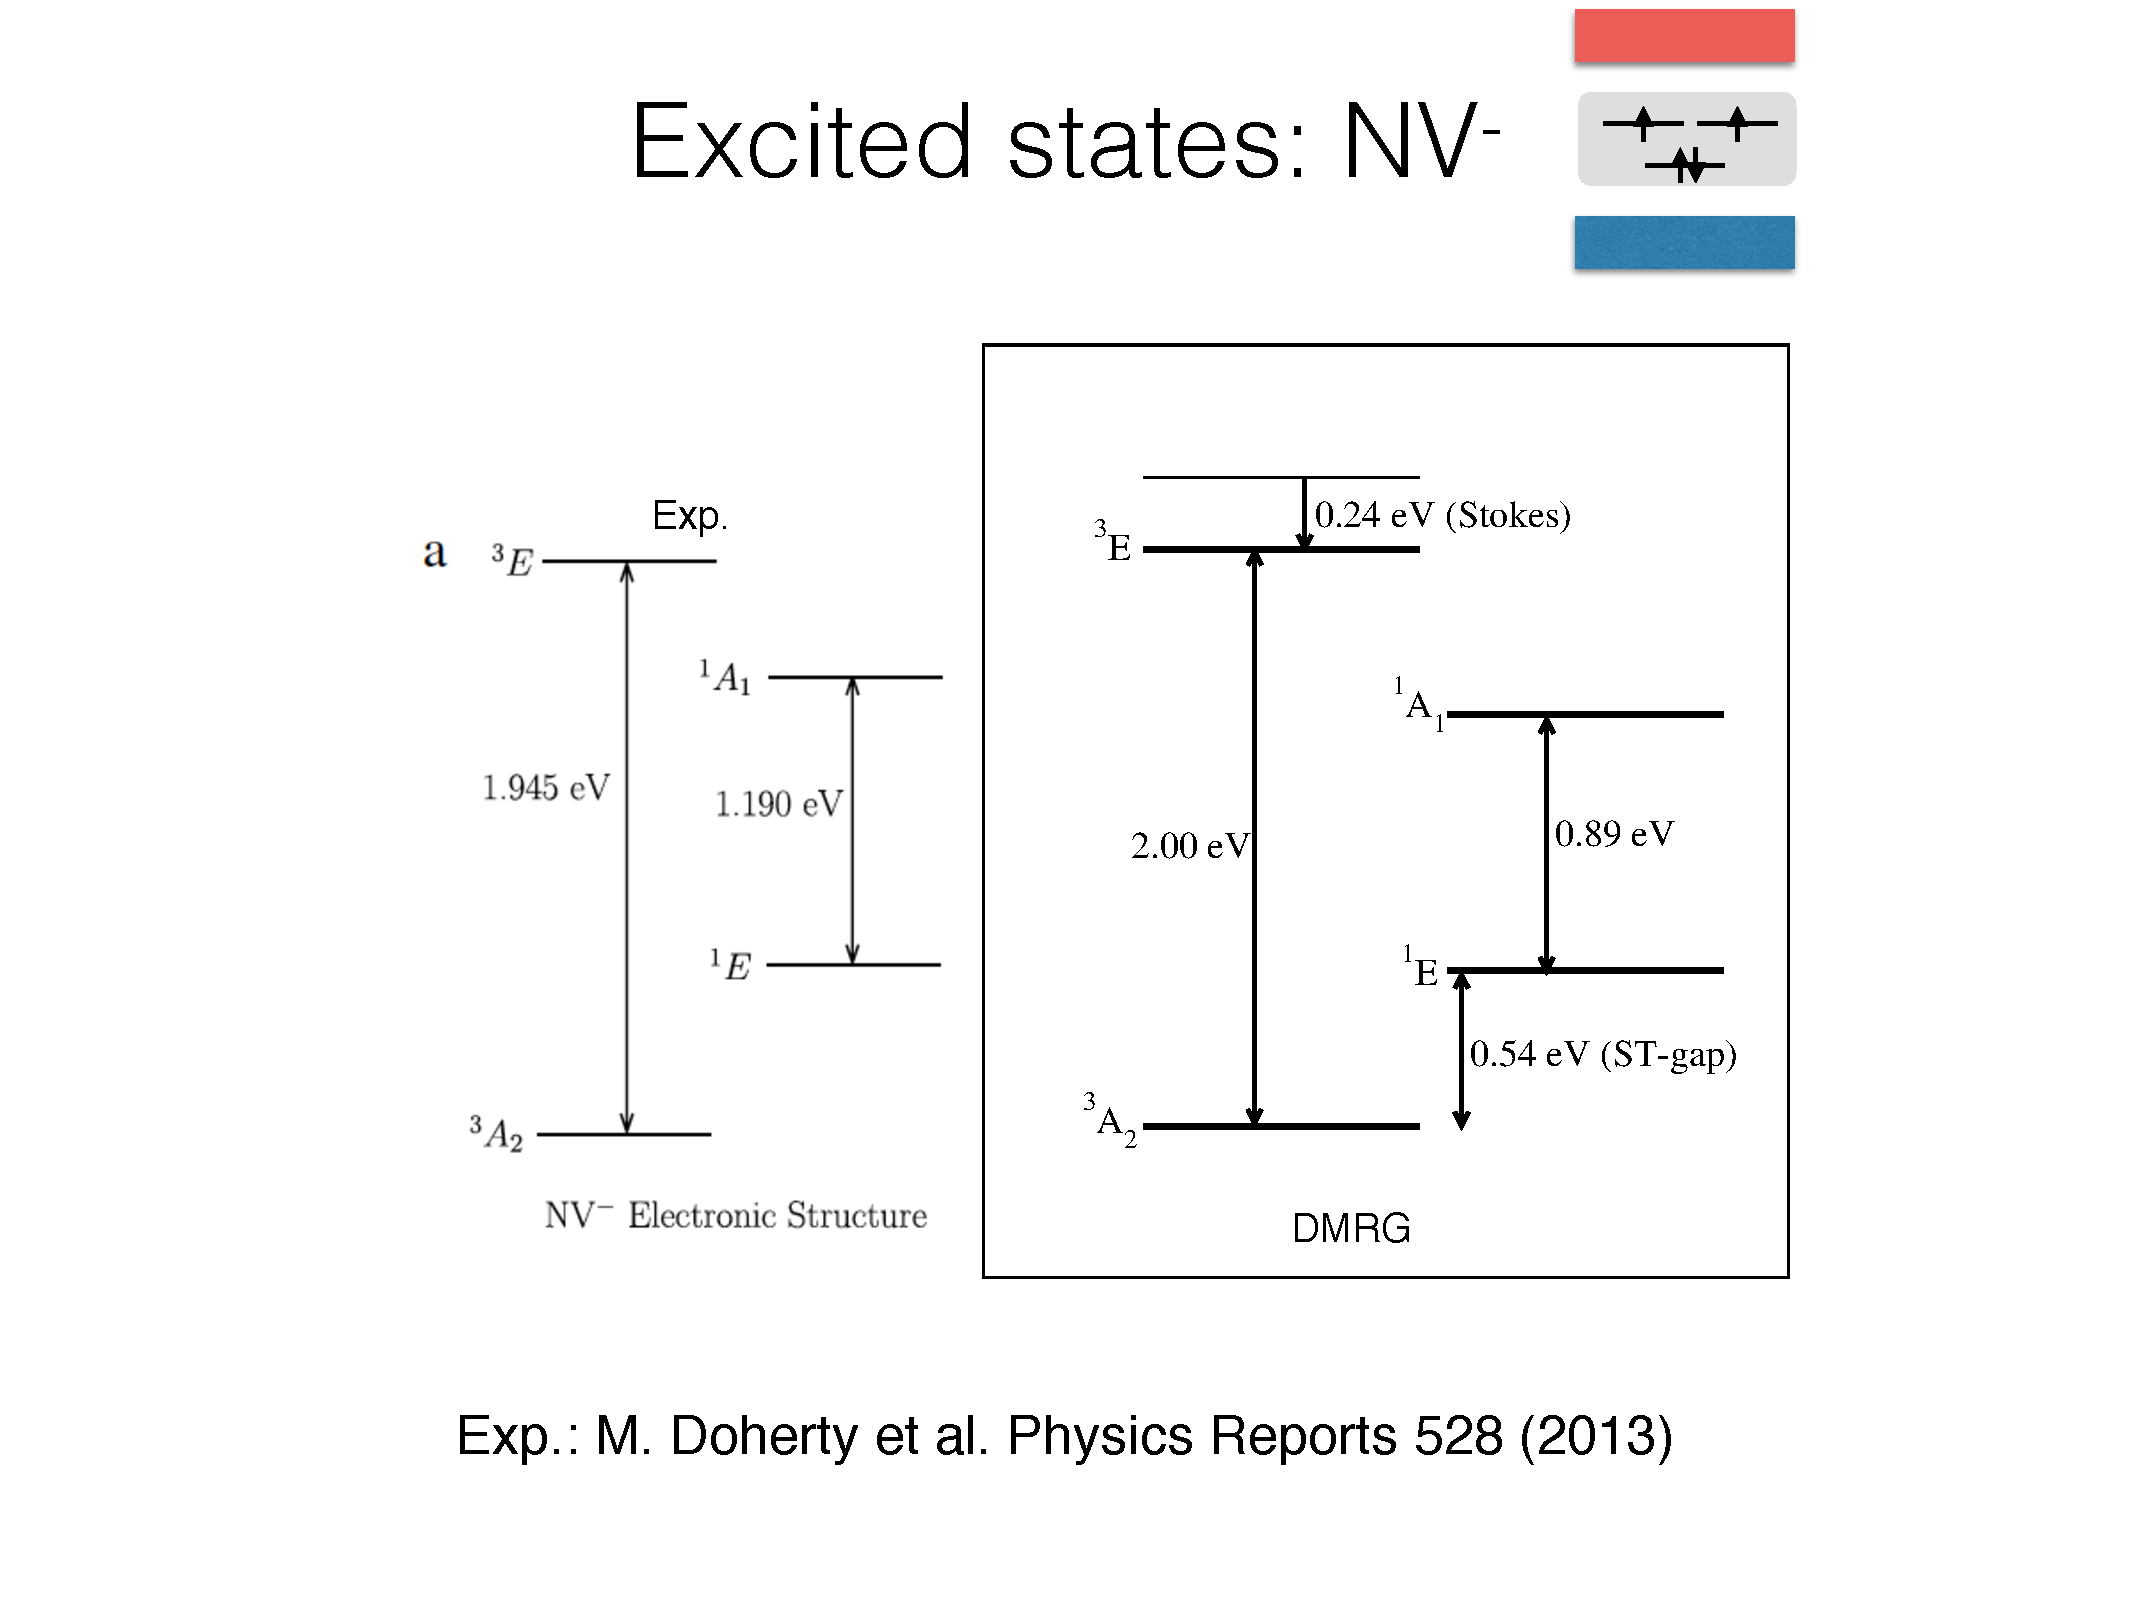
\includegraphics[width=0.5\textwidth, trim=220 200 570 220, clip]{figures/dmrg_results.pdf}
    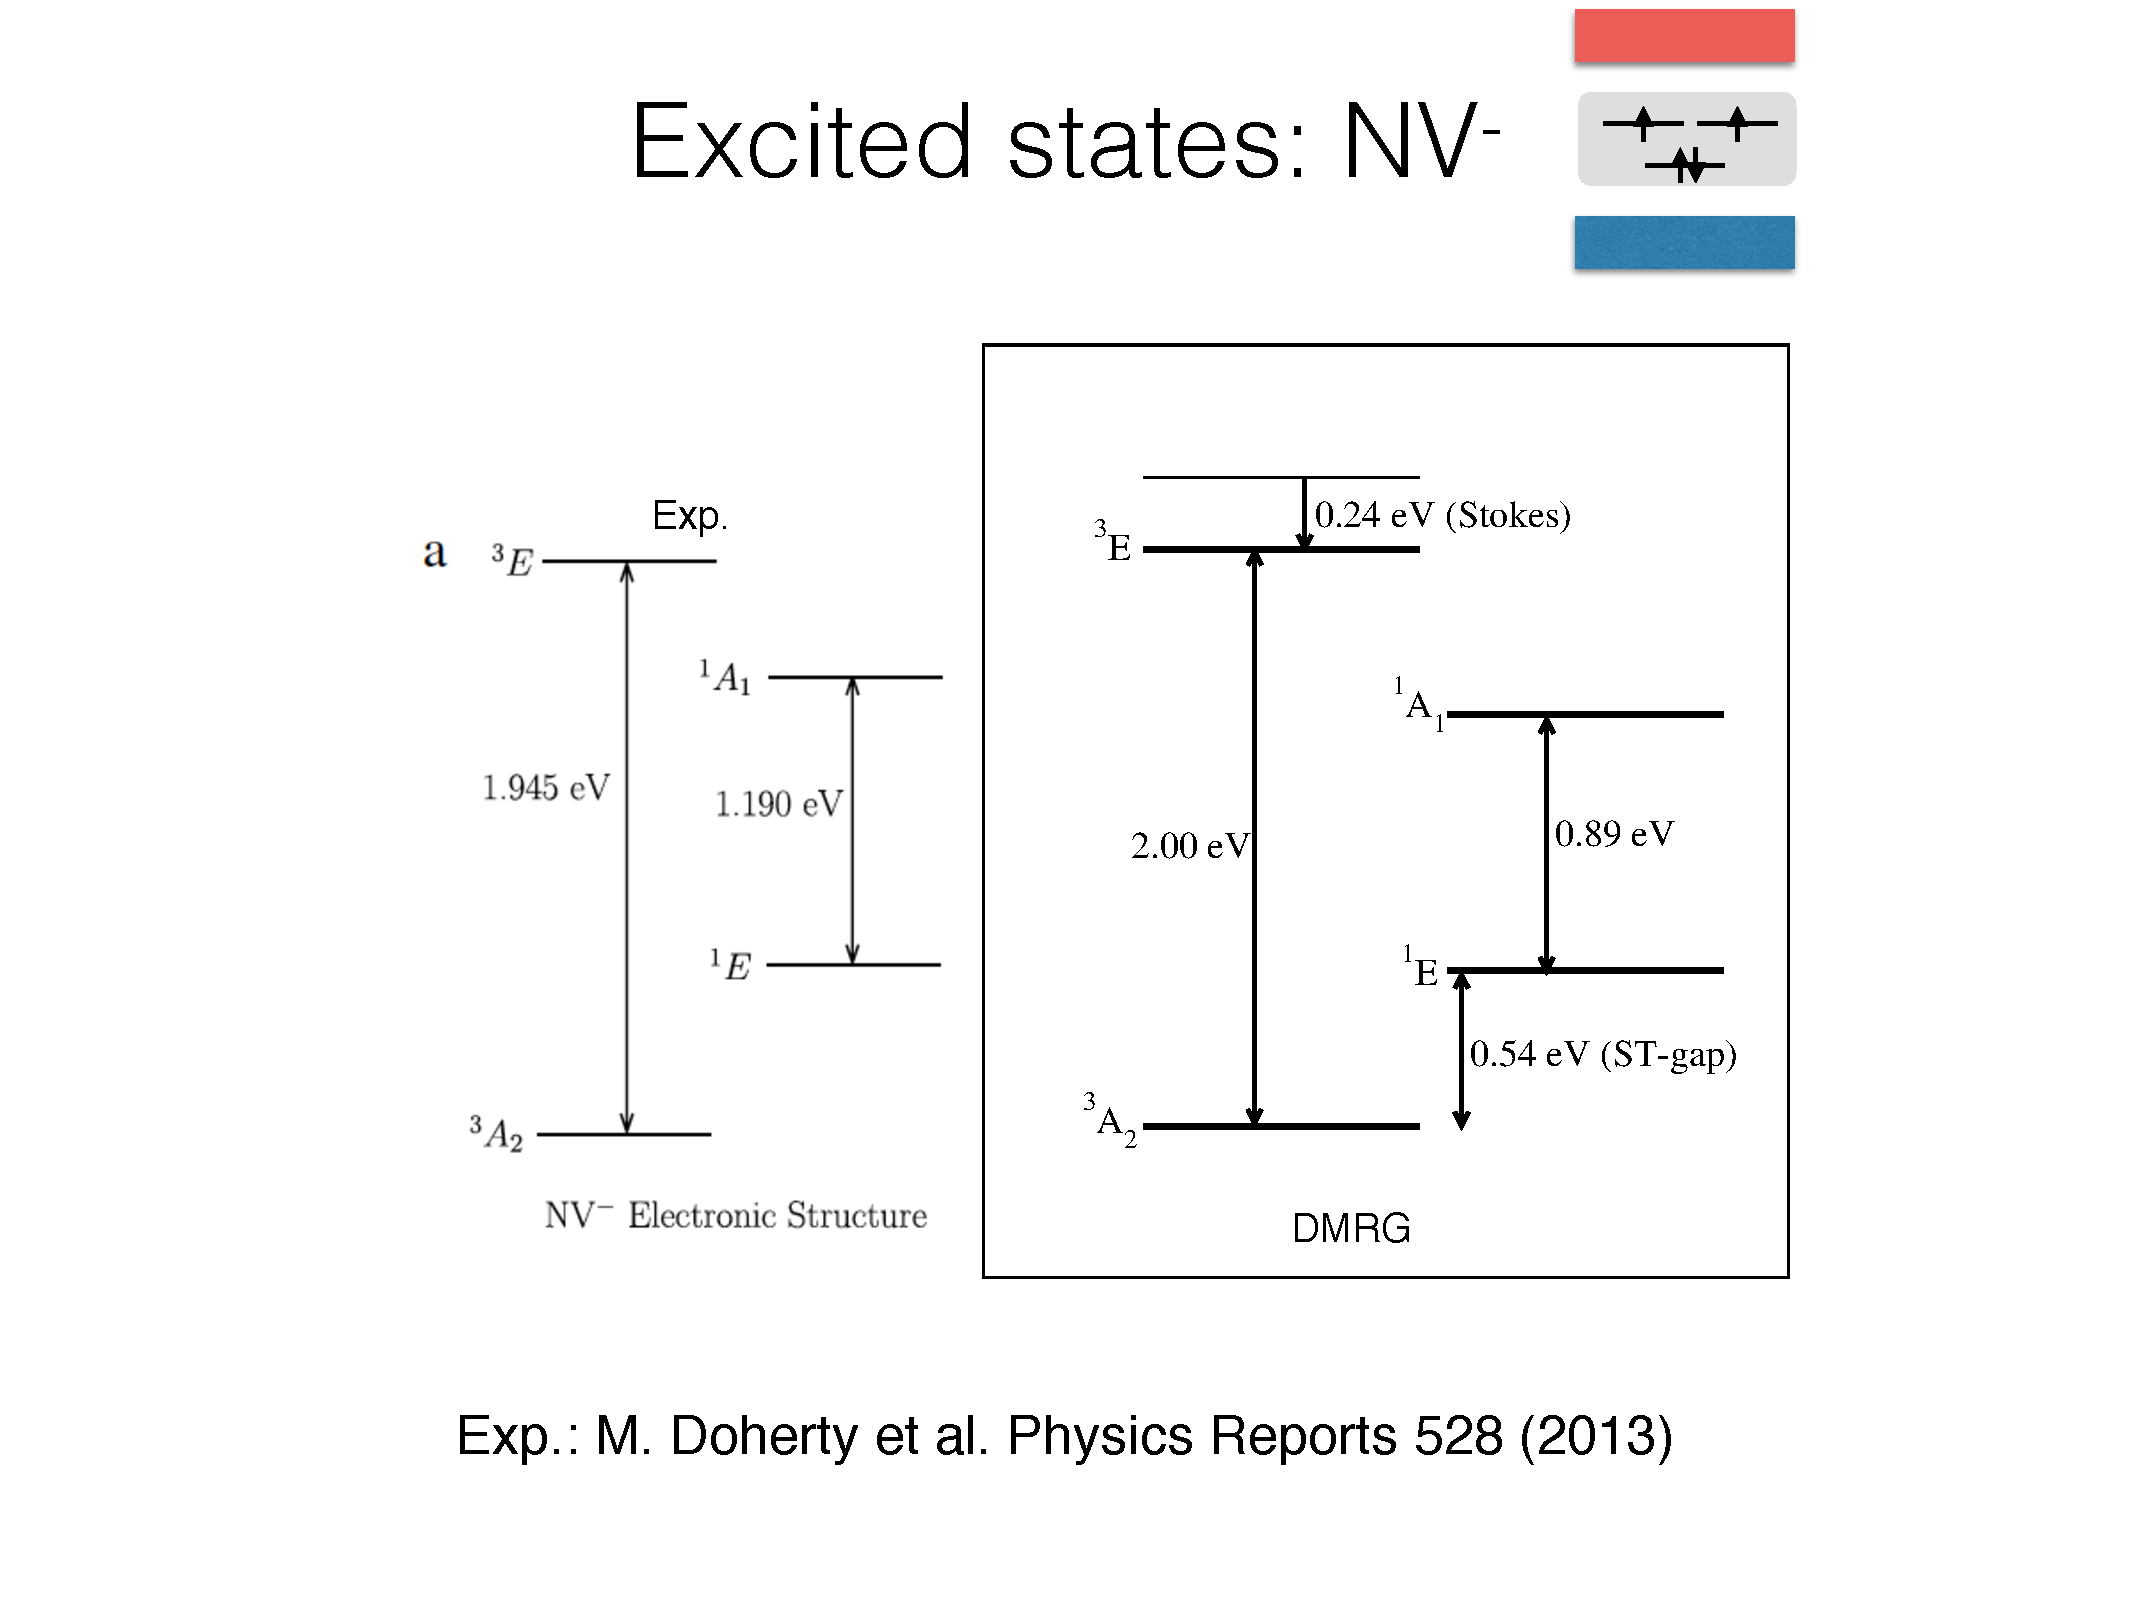
\includegraphics[width=0.6\textwidth, trim=500 200 190 200, clip]{figures/dmrg_results.pdf}
  \end{center}
}


%  Details {{{1  %
%%%%%%%%%%%%%%%%%%
\headerbox{\it Computational details}{
  name=computational-details,
  column=2,
  span=1,
  below=dmrg}{
  \begin{itemize}
    \item Calculations performed using VASP.
    \item \emph{DMRG} calculations
      done using S. Sharma and G. Chan \textit{Block} code.
    \item Plane waves basis set.
    \item PBE exchange-correlation functional.
    \item Unit cell size of 128 atoms.
    \item VASP zero field splitting implementation.
    %\item Calculation of states $ A $ and $ C $ performed with lattice relaxation.
      %$ B $  and $ D $  were respectively calculated with the relaxed structure of $ A $ and $ C $.
      %\vspace{.15cm}
  \end{itemize}
}



%  Discussion {{{1  %
%%%%%%%%%%%%%%%%%%%%%
\headerbox{\it Discussion}{
  name=abcd-details,
  column=0,
  span=3,
  below=computational-details
  }{
  \begin{minipage}{0.2\textwidth}
    \centering
    %\includegraphics[height=1.7\textwidth]{figures/lumos.pdf}
    %\includegraphics[height=1.7\textwidth]{figures/lumos/128_definitiv_1_NV_minus.pdf}
    %{figures/simple_orbital_pictures/basic_level_definition_with_spin_3.tex}
    %\includegraphics[height=1.7\textwidth]{figures/simple_orbital_pictures/basic_level_definition_with_spin_3.pdf}
  \end{minipage}
  \begin{minipage}{0.75\textwidth}
    \begin{itemize}
      \item Prediction of new types of defects by studying diamond allotropes
        with and negatively charged NV center as a test case.
      \item
        Calculation of defect fingerprints such as the spin-spin interaction parameters
        $ E $ and $ D $.
      \item
        Calculation of $ \mathrm{NV}^{-} $ excited states self-consistently
        by interfacing VASP with Block.
    \end{itemize}
    {\smaller\ [1] M. Doherty et al, The nitrogen-vacancy colour centre in diamond, arXiv:1302.3288. }
  \end{minipage}
}






\end{poster}

\end{document}

% vim:spell ft=tex nospell fdm=marker:
